\newpage
\clearpage
\section{Segmentação de Imagens}
\label{segment:image}

O processo de segmentação de imagens pertence às áreas de visão computacional e processamento digital de imagens, sendo seu objetivo principal a distinção de áreas ou propriedades desejadas \cite{Haralick1985, Yuheng2017, Ghosh2019} de uma determinada imagem, assim, sendo possível realizar análises mais precisas ou separar apenas as áreas que são convenientes e de interesse, de acordo com o objetivo da análise.

A partir de segmentações de imagens é possível realizar tarefas de reconhecimento, que são muito utilizadas para áreas de reconhecimento facial \cite{Yuheng2017}, por exemplo. Além dessa, dentre outras grandes áreas para a aplicação das técnicas de segmentação de imagens destacam-se setores da medicina, pavimentações, pedestres, carros autônomos, sensoriamento remoto e afins. Para exemplificar, as Figuras \ref{segment:fig:1}\subref{segment:fig:1.1} e \ref{segment:fig:1}\subref{segment:fig:1.2} representam segmentações faciais e médicas, respectivamente.  

\begin{figure}[H]
   \caption{Exemplos de segmentações de imagens.}
   \centering
   \label{segment:fig:1}
    \begin{subfigure}[t]{0.5\textwidth}
        \centering
        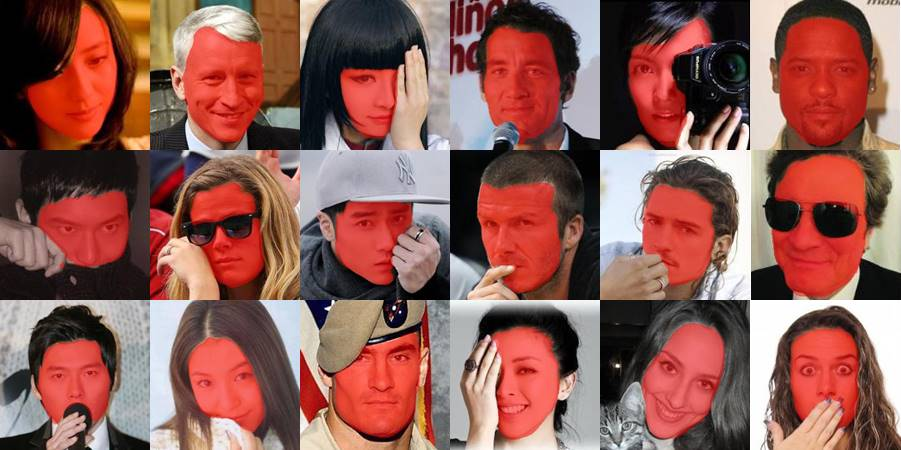
\includegraphics[width=1\linewidth]{recursos/imagens/image_seg/faces.png}
        \caption{Segmentação de imagens faciais.}
        \label{segment:fig:1.1}
    \end{subfigure}%
    ~ 

    \begin{subfigure}[t]{0.5\textwidth}
        \centering
        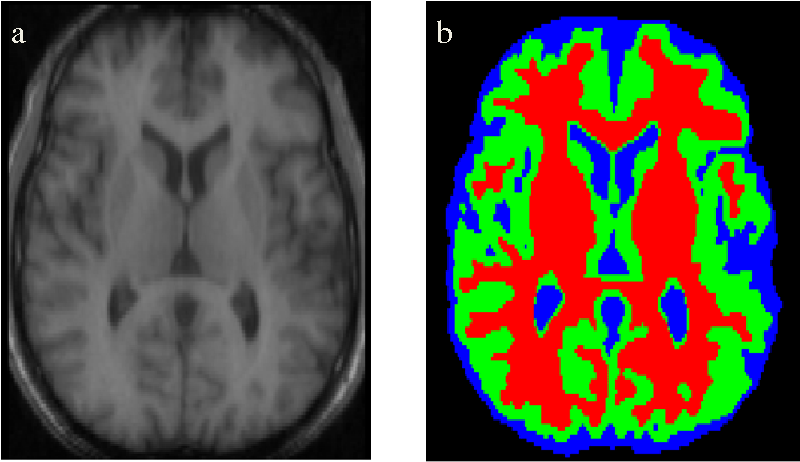
\includegraphics[width=1\linewidth]{recursos/imagens/image_seg/cerebro.png}
        \caption{Segmentação de imagem médica.}
        \label{segment:fig:1.2}
    \end{subfigure}%
    ~

    \vspace*{1 cm}
    Fonte: \cite{Nirkin2018} e \cite{Withey2008}, respectivamente.
\end{figure}

Assim, estando claro o conceito de segmentação de imagens, diversas técnicas são estudadas nessa área, tendo que às tradicionais são citadas na Seção \ref{segment:segment}.


\subsection{Métodos e Técnicas Tradicionais}
\label{segment:segment}

Quando se trata de segmentações, algumas técnicas são muito conhecidas e utilizadas, sendo que algumas são calculas utilizando apenas convoluções matriciais simples \cite{Yuheng2017}.

Sendo assim, nas próximas seções algumas técnicas de segmentação serão discutidas, das quais pode-se citar as segmentações baseadas em regiões (Seção \ref{segment:region}), bordas  (Seção \ref{segment:limit}), agrupamentos  (Seção \ref{segment:group}) e até mesmo as que fazem uso de redes neurais  (Seção \ref{segment:neural}).

\subsubsection{Segmentação Baseada em Regiões}
\label{segment:region}

Alguns tipos de segmentação comumente trabalham com os valores dos pixels, de modo que seja possível segregar áreas e regiões de interesse de regiões que não são possuem relevância. Dentre as diversas técnicas, vale destacar a técnica de \textit{Threshold Segmentation}, ou em português, segmentação limiar, a qual é desenvolvida e aplicada em diversos trabalhos \cite{Yanowitz1989}.

De um modo geral, a segmentação por meio da determinação de um limiar acontece em imagens que utilizam a escala de cinza ou algum sistema de cor que possua um canal voltado para intensidade, como o sistema HSV \cite{schneider2003experimentos}, visto que quando no sistema correto, há a determinação de um valor entre a o fundo e a área de interesse da imagem. Dessa forma, os pixels acima do valor médio determinado são categorizados como área de intensidade e os inferiores são categorizados como fundo \cite{pedrini2008analise}, como é possível observar na Equação \ref{segment:eq:1}, em que $T$ representa o limiar determinado, $f(x,y)$ o pixel da imagem $f$ e $g(x,y)$ o pixel limiarizado:

\begin{equation}
\label{segment:eq:1}
    g(x,y) = \left\{\begin{matrix}
        0, & se & f(x,y) \leq T\\ 
        1, & se & f(x,y) > T
    \end{matrix}\right
    ..
\end{equation}

Sobre \textit{Threshold Segmentation}, vale citar que há uma série de técnicas para determinar o valor de limiarização como é trabalhado por \cite{Al-amri2010}, mas habitualmente utiliza-se da média \cite{Al-amri2010, Yanowitz1989, Yuheng2017} ou de técnicas adaptativas que são citadas em trabalhos, como \cite{Yanowitz1989}, mas que ganham repercussões abrangentes e é evidenciada na técnica Otsu \cite{Otsu1979}, principalmente quando se trata de segmentações com um limiar global como demonstra o histograma na Figura \ref{segment:fig:2}\subref{segment:fig:2.1} e o exemplo prático na Figura  \ref{segment:fig:3}\subref{segment:fig:3.3}. Todavia, quando as regiões de interesse estão divididas, faz-se necessário a divisão de limiares locais, como pode ser observado no histograma da Figura \ref{segment:fig:2}\subref{segment:fig:2.2}, Equação \ref{segment:eq:2} ou na Figura \ref{segment:fig:3}\subref{segment:fig:3.4}:

\begin{equation}
\label{segment:eq:2}
    g(x,y) = \left\{\begin{matrix}
        v1, & se & f(x,y) \leq T \\ 
        v2, & se & T_1 < f(x,y) \leq T_2 \\
        v3, & se & f(x,y) > T_2
\end{matrix}\right..
\end{equation}

\begin{figure}[H]
   \caption{Histogramas de limiarizações.}
   \centering
   \label{segment:fig:2}
    \begin{subfigure}[t]{0.45\textwidth}
        \centering
        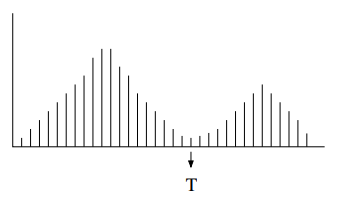
\includegraphics[width=0.5\linewidth]{recursos/imagens/image_seg/limi_glob.png}
        \caption{Histograma de limiarização global.}
        \label{segment:fig:2.1}
    \end{subfigure}%
    ~ 
    \begin{subfigure}[t]{0.45\textwidth}
        \centering
        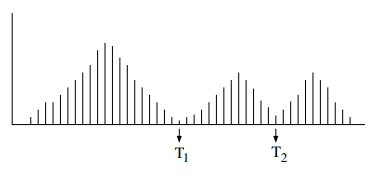
\includegraphics[width=0.5\linewidth]{recursos/imagens/image_seg/limi_local.png}
        \caption{Histograma de limiarização local.}
        \label{segment:fig:2.2}
    \end{subfigure}%

    \vspace*{1 cm}
    Fonte: retirado de \cite{pedrini2008analise}.
\end{figure}

\begin{figure}[H]
   \caption{Limiarizações.}
   \centering
   \label{segment:fig:3}
    \begin{subfigure}[t]{0.45\textwidth}
        \centering
        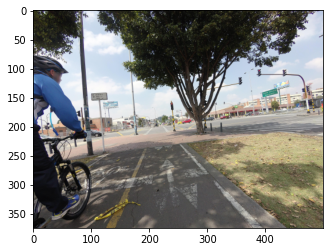
\includegraphics[height=1.5in]{recursos/imagens/image_seg/mapi.png}
        \caption{Imagem original.}
        \label{segment:fig:3.1}
    \end{subfigure}%
    ~ 
    \begin{subfigure}[t]{0.45\textwidth}
        \centering
        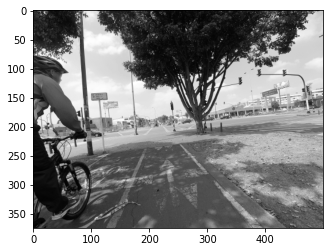
\includegraphics[height=1.5in]{recursos/imagens/image_seg/gray_mapi.png}
        \caption{Imagem em escala de cinza.}
        \label{segment:fig:3.2}
    \end{subfigure}%
    ~ 
    
    \begin{subfigure}[t]{0.45\textwidth}
        \centering
        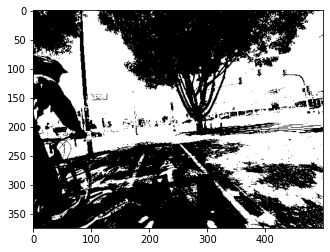
\includegraphics[height=1.5in]{recursos/imagens/image_seg/bw_mapi.png}
        \caption{Imagem limiarizada globalmente.}
        \label{segment:fig:3.3}
    \end{subfigure}
    ~
    \begin{subfigure}[t]{0.45\textwidth}
        \centering
        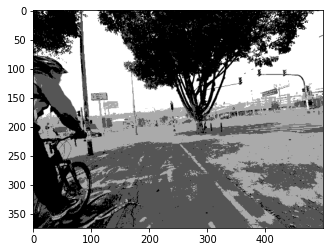
\includegraphics[height=1.5in]{recursos/imagens/image_seg/local_mapi.png}
        \caption{Imagem limiarizada localmente.}
        \label{segment:fig:3.4}
    \end{subfigure}

    \vspace*{1 cm}
    Fonte: retirado e adaptado de \cite{Neuhold2017_ICCV}.
\end{figure}

Por fim, ainda sobre a segmentação baseada em regiões, uma das técnicas que também se destaca é a de crescimento de regiões, ou em inglês, \textit{Region Growning}. Essa técnica consiste em traçar um limiar e distribuir sementes na imagem, de modo que os pixels vizinhos sejam transformados pelo valor da semente quando com diferença inferiores ao limiar determinado, sendo possível visualizar tal ocorrência a partir da Figura \ref{segment:fig:4} ou por meio da Equação \ref{segment:eq:3}, sendo $P(R)$ o predicado da região, $f(r,s)$ o pixel semente, e $f(x,y)$ o pixel vizinho ao da semente por vizinhança-8:

\begin{figure}[H]
   \caption{Crescimento de região.}
   \centering
   \label{segment:fig:4}
    \begin{subfigure}[t]{0.45\textwidth}
        \centering
        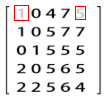
\includegraphics[height=1.5in]{recursos/imagens/image_seg/m1.png}
        \caption{Imagem original, sendo em vermelho os pixels sementes ($f(r,s)$).}
        \label{segment:fig:4.1}
    \end{subfigure}
    ~ 
    \begin{subfigure}[t]{0.45\textwidth}
        \centering
        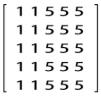
\includegraphics[height=1.5in]{recursos/imagens/image_seg/m2.png}
        \caption{Crescimento de região com $T = 3$.}
        \label{segment:fig:4.2}
    \end{subfigure}
    ~ 

    \begin{subfigure}[t]{0.45\textwidth}
        \centering
        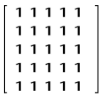
\includegraphics[height=1.5in]{recursos/imagens/image_seg/m3.png}
        \caption{Crescimento de região com $T = 6$.}
        \label{segment:fig:4.3}
    \end{subfigure}

    \vspace*{1 cm}
    Fonte: retirado e adaptado de \cite{Yuheng2017}.
\end{figure}

\begin{equation}
\label{segment:eq:3}
P(R) = \left\{\begin{matrix}
    VERDADEIRO, & se |f(x,y) - f(r,s)| \leq T \\
    FALSO,      &  \text{caso contrário}
\end{matrix}\right..
\end{equation}

Por fim, ainda sobre o aspecto de crescimento de região, salienta-se que é de extrema importância a determinação das sementes e do valor limiar \cite{Yuheng2017, pedrini2008analise}, além de ser necessário ter as condições para determinação de sistema de cores e canais semelhantes às de \textit{threshold segmentation}.


\subsubsection{Segmentação por Bordas}
\label{segment:limit}

Em meio às categorias de segmentação tradicional estão as segmentações por descontinuidade, com subcategorias de segmentação por pontos, retas, junções e, finalmente, por bordas \cite{pedrini2008analise}. Correntemente, é a partir dessas segmentações que são construídos os filtros convolucionais que foram explorados na Seção \ref{deep:CNN}.

Sendo assim, é de referir que as bordas são definidas como limites que possuem regiões com contrastes discrepantes em relação ao seus níveis de cinza  ou que separam duas regiões homogêneas \cite{pedrini2008analise,Yuheng2017}, algo que não é tão perceptível em imagens reais, considerando o fato de que os dispositivos de captura costumeiramente realizam a suavização e o borramento das bordas.

Para as questões de detecção dessas bordas são utilizados cálculos de derivadas, assim  como a representação por meio de matrizes de filtros se fazem comuns \cite{pedrini2008analise, muthukrishnan2011edge}, citando que um dos mais conhecidos filtros de primeira ordem é o filtro Sobel e para segunda ordem, cita-se o filtro laplaciano.

O operador Sobel, em suma, pode ser introduzido ao assimilar com uma operação de média local, em que este pode calcular bordas horizontais e verticais ou realizar a combinação de ambas. Tendo que diferenças horizontais entre os pontos são utilizadas para detecção de bordas verticais e que diferenças verticais entre os pontos são usadas para detecção de bordas horizontais \cite{pedrini2008analise}.

Essas operações de Sobel podem ser feitas com o auxilio de convoluções e das seguintes matrizes nas Equações \ref{segment:eq:4} e \ref{segment:eq:5}:

\begin{equation}
\label{segment:eq:4}
    G_x = \begin{bmatrix}
    -1 & 0 & 1 \\ 
    -2 & 0 & 2 \\ 
    -1 & 0 & 1
    \end{bmatrix}
\end{equation}
e
\begin{equation}
\label{segment:eq:5}
    G_y = \begin{bmatrix}
    -1 & -2 & -1 \\ 
     0 & 0 & 0 \\ 
     1 & 2 & 1
    \end{bmatrix},
\end{equation}
sendo $G_x$ uma matriz $3x3$ para o encontro de bordas verticais e $G_y$ para o encontro de bordas horizontais \cite{pedrini2008analise}, tendo que sua combinação pode resultar em imagens como a da Figura \ref{segment:fig:7}.

\begin{figure}[H]
    \caption{Segmentação com operador Sobel.}
    \centering
    \label{segment:fig:7}
    \begin{subfigure}[t]{0.45\textwidth}
        \centering
        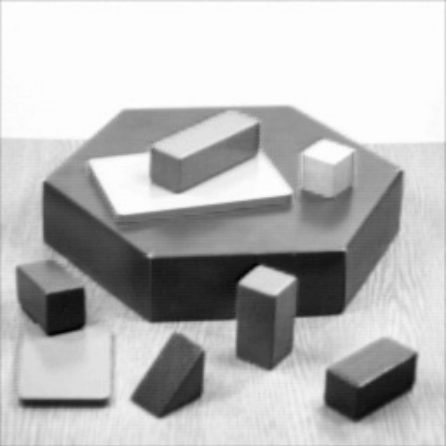
\includegraphics[height=1.3in]{recursos/imagens/image_seg/o1.png}
        \caption{Imagem original.}
        \label{segment:fig:7.1}
    \end{subfigure}%
    ~ 
    \begin{subfigure}[t]{0.45\textwidth}
        \centering
        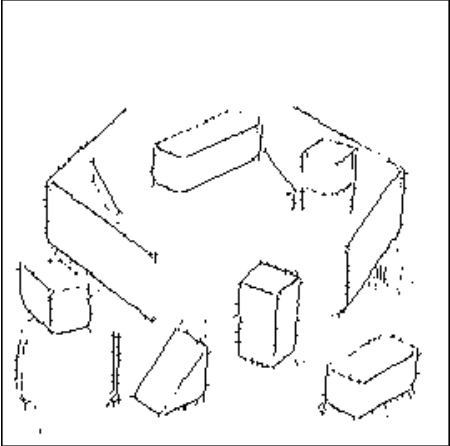
\includegraphics[height=1.3in]{recursos/imagens/image_seg/o2.png}
        \caption{Imagem resultante de $G_x$.}
        \label{segment:fig:7.2}
    \end{subfigure}%
    ~ 
    
    \begin{subfigure}[t]{0.45\textwidth}
        \centering
        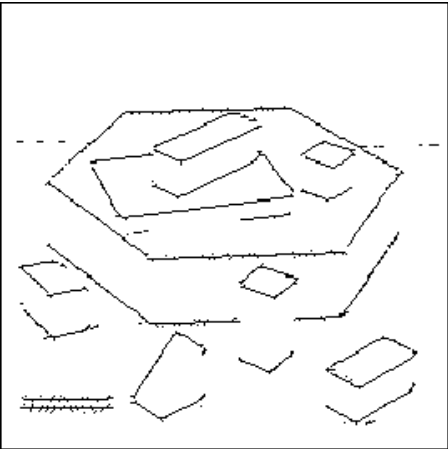
\includegraphics[height=1.3in]{recursos/imagens/image_seg/o3.png}
        \caption{Imagem resultante de $G_y$.}
        \label{segment:fig:7.3}
    \end{subfigure}
    ~
    \begin{subfigure}[t]{0.45\textwidth}
        \centering
        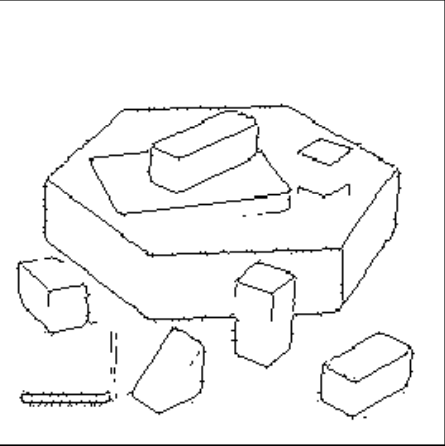
\includegraphics[height=1.3in]{recursos/imagens/image_seg/o4.png}
        \caption{Imagem de combinação entre $G_x$ e $G_y$.}
        \label{segment:fig:7.4}
    \end{subfigure}

    \vspace*{1 cm}
    Fonte: \cite{pedrini2008analise}.
\end{figure}

Já em relação ao \textbf{operador laplaciano}, destaca-se que este faz uso de uma derivada segunda que pode ser representada a partir da Equação \ref{segment:eq:6}:

\begin{equation}
    \label{segment:eq:6}
    \bigtriangledown^2 f = \frac{\partial^2f}{\partial x^2} + \frac{\partial^2f}{\partial y^2},
\end{equation}
tendo que $f(x,y)$ é uma função bidimensional contínua e sendo recomendada para situações em que a imagem não tenha ruído e a posição da borda sejam mais relevantes \cite{Yuheng2017}, isso se dá visto que por contar com uma derivada de segunda ordem, torna-se muito sensível aos ruídos \cite{pedrini2008analise}.

Ainda sobre o operador laplaciano, pode se dizer que há uma necessidade de que o coeficiente do pixel central resulte em um valor positivo e que os seus pixeis externos sejam negativos \cite{pedrini2008analise}, assim, considerando uma matriz de vizinhança-8, pode-se exemplificar uma implementação do operador Laplaciano que considera as derivadas segundas em linhas e colunas tendo por base a matriz $h_1$ (Equação \ref{segment:eq:7}), resultando em aplicações como as visualizadas na Figura \ref{segment:fig:8}, sendo: 

\begin{equation}
    \label{segment:eq:7}
    h_1 = \begin{bmatrix}
     0 &  0 &  0 \\ 
    -1 & -2 & -1 \\ 
     0 &  0 &  0
    \end{bmatrix} +
    \begin{bmatrix}
     0 & -1 & 0 \\ 
     0 &  2 & 0 \\ 
     0 & -1 & 0 
    \end{bmatrix} =
    \begin{bmatrix}
     0 & -1 & 0 \\ 
    -1 &  4 & -1 \\ 
     0 & -1 & 0 
    \end{bmatrix}.
\end{equation}

\begin{figure}[H]
   \caption{Segmentação com operador Laplaciano.}
   \centering
   \label{segment:fig:8}
    \begin{subfigure}[t]{0.45\textwidth}
        \centering
        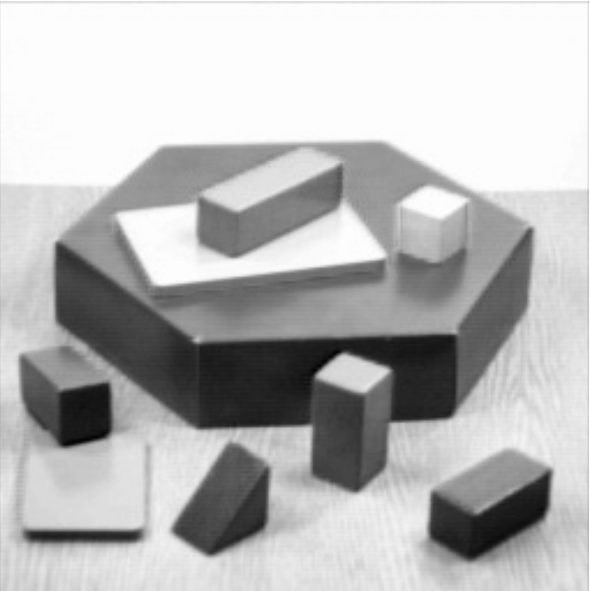
\includegraphics[height=1.5in]{recursos/imagens/image_seg/ol1.png}
        \caption{Imagem original.}
        \label{segment:fig:8.1}
    \end{subfigure}%
    ~ 
    \begin{subfigure}[t]{0.45\textwidth}
        \centering
        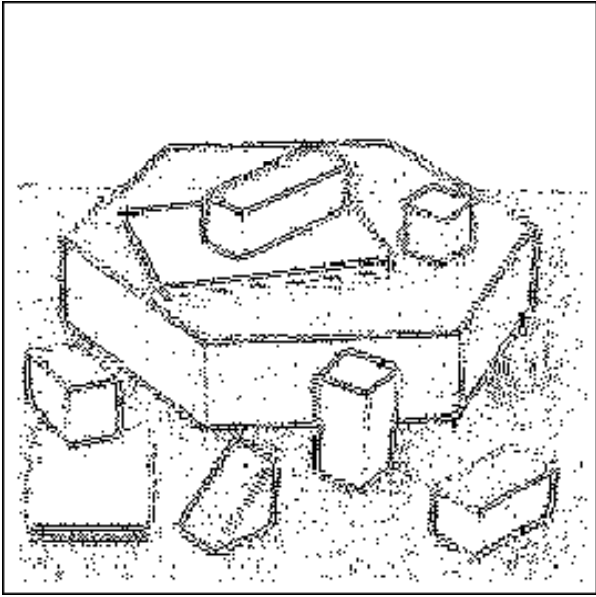
\includegraphics[height=1.5in]{recursos/imagens/image_seg/lp2.png}
        \caption{Mapa de bordas resultante.}
        \label{segment:fig:8.2}
    \end{subfigure}%

    \vspace*{1 cm}
    Fonte: \cite{pedrini2008analise}.
\end{figure}

\subsubsection{Segmentação Baseada em Agrupamentos}
\label{segment:group}

Como o nome propõe, as segmentações baseadas em agrupamentos na esfera de visão computacional e processamento de imagens são compostas pela agregação de pixels que possuem características similares em determinado espaço de características \cite{Yuheng2017}. No entanto, a definição de agrupamento (ou \textit{clustering}) ainda não são concretas \cite{Yuheng2017}, haja vista que não é categorizada como segmentação por alguns autores, pois os agrupamentos são realizados no espaço de medidas, enquanto a segmentação ocorre no domínio espacial da imagem \cite{Haralick1985}.

Posto isso, destaca-se o uso do K-means \cite{macqueen1967some, bock2008origins}, o qual é um método não supervisionado que realiza agrupamento de dados de um \textit{dataset} de acordo com as suas similaridades e em quantidades desejadas ($k$). Ou seja, o algoritmo gera um ponto inicial randômico como centróide para um determinado \textit{cluster} e depois tenta atribuir os demais dados do \textit{dataset} aos \textit{clusters} de acordo com a sua proximidade. Para isso, o algoritmo usa técnicas de distância euclidiana \cite{Mahmud2012}. Vale ressaltar que os pontos centróides são atualizados conforme as classificações que são feitas no algoritmo, e os mesmos param de atualizar quando o algoritmo cumpre seu objetivo de convergência, há poucas interações dos dados com diferentes \textit{clusters} ou através de um número fixo de iterações \cite{dunham2006data}, conforme representado no fluxograma da Figura \ref{segment:fig:6}, tendo que $n \in \mathbb{Z}$.

\begin{figure}[H]
    \centering
    \caption{Fluxograma do algoritmo K-means.}
    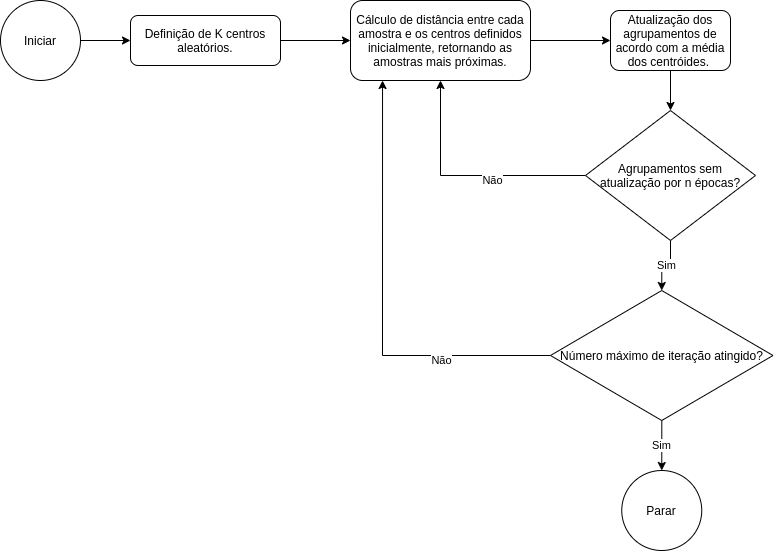
\includegraphics[width=1\linewidth]{recursos/imagens/image_seg/kmeans.png}
    \label{segment:fig:6}

    \vspace*{1 cm}
    Fonte: do próprio autor.
\end{figure}

Na Figura \ref{segment:fig:5}, é possível observar o uso do algoritmo K-means para agrupar as regiões da imagem, tendo que foi definido um valor de $k = 3$.

\begin{figure}[H]
   \caption{Segmentação com K-means.}
   \centering
   \label{segment:fig:5}
    \begin{subfigure}[t]{0.45\textwidth}
        \centering
        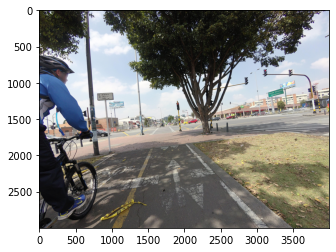
\includegraphics[height=1.5in]{recursos/imagens/image_seg/i1.png}
        \caption{Imagem original.}
        \label{segment:fig:5.1}
    \end{subfigure}%
    ~ 
    \begin{subfigure}[t]{0.45\textwidth}
        \centering
        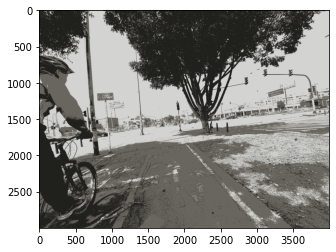
\includegraphics[height=1.5in]{recursos/imagens/image_seg/i2.png}
        \caption{Segmentação com $k = 3$.}
        \label{segment:fig:5.2}
    \end{subfigure}%

    \vspace*{1 cm}
    Fonte: retirado e adaptado de \cite{Neuhold2017_ICCV}.
\end{figure}

\subsubsection{Segmentação com Redes Neurais}
\label{segment:neural}

As segmentações por meio de redes neurais, profundas (Seção \ref{deep:deep}) ou por meio das redes convolucionais (Seção \ref{deep:CNN}) regularmente são confundidas com a área de detecção de objetos \cite{Ghosh2019} pela característica de demarcação e pelo uso das \textit{bounding box}. Não obstante vale destacar que para segmentações de imagens as redes mais utilizadas são as CNNs, de modo que esta consegue trabalhar com a extração das características mais importantes de determinada imagem e, em seguida, organizá-las, sendo eficiente não somente em tarefas de detecção, localização e rastreamento de objetos, mas também, como neste caso, segmentação de imagens \cite{Ghosh2019}.

Métodos mais modernos que seguem essa linha serão explicados detalhadamente nos capítulos \ref{semantic:semantic}, \ref{instance:instance} e \ref{panoptic:panoptic}.


\subsection{Considerações Finais do Capítulo}
\label{segment:conclusion}

Na Tabela \ref{segment:table:1}, é possível visualizar as técnicas comentadas no decorrer do capítulo, assim como uma breve descrição de seus usos, suas vantagens e desvantagens.

\begin{table}[H]
\centering
\caption{Comparação entre os métodos de segmentações tradicionais.}
\label{segment:table:1}
\resizebox{\textwidth}{!}{%

    \begin{tabular}{l|l|l|l}
    \textbf{Técnica}                    & \textbf{Descrição}                                                                                                                                    & \textbf{Vantagens}                                                                                                                                                                                                     & \textbf{Desvantagens}                                                                                                                                                                        \\ 
    \hline
    Segmentação Baseada em Regiões      & \begin{tabular}[c]{@{}l@{}}Concentra-se em encontrar e\\agrupar valores semelhantes\\sendo separados por um limiar.\end{tabular}                      & \begin{tabular}[c]{@{}l@{}}- Possui baixa complexidade\\~e alto desempenho;\\ - Não requer pré-processamento;\\ - Recomendado para imagens\\~com alto contraste entre fundo e\\~objeto de interesse.\end{tabular}      & \begin{tabular}[c]{@{}l@{}}- Omissão de detalhes quando não\\~há um contraste significante.\end{tabular}                                                                                     \\ 
    \hline
    Segmentação por Bordas              & \begin{tabular}[c]{@{}l@{}}Realizado com base na\\detecção de descontinuidade,\\detectando bordas e definindo\\um limite do objeto.\end{tabular}      & \begin{tabular}[c]{@{}l@{}}- Recomendável para imagens\\~com bons contrastes entre\\~os objetos.\end{tabular}                                                                                                          & \begin{tabular}[c]{@{}l@{}}- Perda de detalhes para imagens\\~com muitas bordas, ruidosas ou\\~com baixo contraste entre os objetos.\end{tabular}                                            \\ 
    \hline
    Segmentação Baseada em Agrupamentos & \begin{tabular}[c]{@{}l@{}}Divide os pixels da imagem\\em k \textit{clusters} homogêneos e\\exclusivos obtendo, assim,\\as segmentações.\end{tabular} & \begin{tabular}[c]{@{}l@{}}- Conceitos já estabelecido;\\ - Recomendado para aplicações\\~em tempo real;\\ - Bom desempenho para pequenos\\~\textit{datasets};\\ - Não precisa de tempo de\\~treinamento.\end{tabular} & \begin{tabular}[c]{@{}l@{}}- Pode demandar muito tempo para\\~encontrar a minimização da função\\~de custo;\\ - Não é adequado para agrupar \\\textit{~clusters} não convexos.\end{tabular}  \\ 
    \hline
    Segmentação com Redes Neurais       & \begin{tabular}[c]{@{}l@{}}Normalmente relacionada\\a algoritmos de aprendizado\\profundo e CNNs.\end{tabular}                                        & \begin{tabular}[c]{@{}l@{}}- Conceito já estabelecido;\\ - Abordagem simples e flexível.\end{tabular}                                                                                                                  & \begin{tabular}[c]{@{}l@{}}- O treinamento do modelo pode\\~consumir muito tempo e recursos.\end{tabular}                                                                                    \\
    \hline
    \end{tabular}
}

\vspace*{1 cm}
Fonte: do próprio autor.
\end{table}

Na Seção \ref{segment:segment}, foi comentado sobre os algoritmos comumente utilizados para segmentações, trabalhando desde algoritmos mais simples como o de \textit{threshold segmentation} (Seção \ref{segment:region}) até o nível de complexidade de técnicas de redes neurais artificiais (Seção \ref{segment:neural}). Porém como comentado por \cite{Ghosh2019} e por \cite{Minaee2021}, hodiernamente há segmentações que utilizam de \textit{deep learning} e possuem ótimas abordagens, as quais estamos denominando como segmentações modernas e serão exploradas nas próximas seções.